% !Mode:: "TeX:UTF-8"
% !TEX program = xelatex


%%%%%%%%%% Port for Win %%%%%%%%%%%
% Modified: Cheng Hong

\def\usewhat{xelatex}
\documentclass[12pt,openany,oneside]{ctexbook}

% ------- 章节编号改为阿拉伯数字（CTeX v2 语法） -------
\ctexset{
  chapter/name = {},        % 去掉“第”
  chapter/number = \arabic{chapter},  % 阿拉伯数字编号
  chapter/format = \thechapter        % 只显示“1”，“2”不带“章”
}
% -------------------------------------------------------

% ------- 取消 \chapter 自动换页 -------
\makeatletter
\renewcommand{\chapter}{%
  \@afterindentfalse
  \secdef\@chapter\@schapter}
\makeatother
% -----------------------------------

% !Mode:: "TeX:UTF-8"

%%%%%%%%%% Package %%%%%%%%%%%%
\usepackage{CJK}
\usepackage{lmodern}
\usepackage[T1]{fontenc}
\usepackage{graphicx}                       % 支持插图处理
\usepackage[a4paper,text={146.4true mm,239.2 true mm},top= 25.4 true mm, bottom= 25.4 true mm,
                                                    bindingoffset=10 true mm, % 装订线的偏移量
                                                    left=31.7 true mm,right=31.7 true mm,
                                                    head=6true mm,headsep=6.5true mm,foot=16.5 true mm]{geometry}
                                            % 支持版面尺寸设置 设置页面大小
\usepackage[squaren]{SIunits}               % 支持国际标准单位
\usepackage{makecell}                      % 支持表格中的单元格换行
\usepackage{titlesec}                       % 控制标题的宏包
\usepackage{titletoc}                       % 控制目录的宏包
\usepackage{fancyhdr}                       % fancyhdr宏包 支持页眉和页脚的相关定义
%\usepackage{ctex}                     % 支持中文显示
\usepackage{CJKpunct}                       % 精细调整中文的标点符号
\usepackage{color}                          % 支持彩色
\usepackage{amsmath}                        % AMSLaTeX宏包 用来排出更加漂亮的公式
\usepackage{amssymb}                        % 数学符号生成命令
\usepackage[below]{placeins}    %允许上一个section的浮动图形出现在下一个section的开始部分,还提供\FloatBarrier命令,使所有未处理的浮动图形立即被处理
\usepackage{multirow}                       % 使用Multirow宏包，使得表格可以合并多个row格
\usepackage{booktabs}                       % 表格，横的粗线；\specialrule{1pt}{0pt}{0pt}
\usepackage{longtable}                      % 支持跨页的表格。
\usepackage{tabularx}                       % 自动设置表格的列宽
\usepackage{subfigure}                      % 支持子图 %centerlast 设置最后一行是否居中
\usepackage[subfigure]{ccaption}            % 支持子图的中文标题
\usepackage[sort&compress,numbers]{natbib}  % 支持引用缩写的宏包
\usepackage{enumitem}                       % 使用enumitem宏包,改变列表项的格式
\usepackage{calc}                           % 长度可以用+ - * / 进行计算
\usepackage{txfonts}                        % 字体宏包
\usepackage{bm}                             % 处理数学公式中的黑斜体的宏包
\usepackage[amsmath,thmmarks,hyperref]{ntheorem}  % 定理类环境宏包，其中 amsmath 选项用来兼容 AMS LaTeX 的宏包
\usepackage{CJKnumb}                        % 提供将阿拉伯数字转换成中文数字的命令
\usepackage{indentfirst}                    % 首行缩进宏包
\usepackage{CJKutf8}                        % 用在UTF8编码环境下，它可以自动调用CJK，同时针对UTF8编码作了设置
%\usepackage{hypbmsec}                      % 用来控制书签中标题显示内容
\newcommand{\tabincell}[2]{\begin{tabular}{@{}#1@{}}#2\end{tabular}}
\usepackage{xcolor}
%支持代码环境
\usepackage{listings}
\lstset{numbers=left,
language=[ANSI]{C},
numberstyle=\tiny,
extendedchars=false,
showstringspaces=false, 
breakatwhitespace=false,
breaklines=true,
captionpos=b,
keywordstyle=\color{blue!70},
commentstyle=\color{red!50!green!50!blue!50},
frame=shadowbox,
rulesepcolor=\color{red!20!green!20!blue!20}
}
%支持算法环境
\usepackage[boxed,ruled,lined]{algorithm2e}
\usepackage{algorithmic}

\usepackage{array}
\newcommand{\PreserveBackslash}[1]{\let\temp=\\#1\let\\=\temp}
\newcolumntype{C}[1]{>{\PreserveBackslash\centering}p{#1}}
\newcolumntype{R}[1]{>{\PreserveBackslash\raggedleft}p{#1}}
\newcolumntype{L}[1]{>{\PreserveBackslash\raggedright}p{#1}}

\def\atemp{xelatex}\ifx\atemp\usewhat
% \usepackage[unicode, % 支持Unicode字符
%             pdfstartview=FitH, % 设置PDF打开时的视图
%             bookmarksnumbered=true, % 设置书签
%             bookmarksopen=true, % 设置书签
%             colorlinks=false, % 设置链接颜色
%         %     pdfborder={0 0 1},  % 设置链接边框
%             pdfborder={0 0 0},  % 隐藏链接边框
%             citecolor=blue, % 设置引用颜色
%             linkcolor=red, % 设置引用颜色
%             anchorcolor=green, % 设置锚点颜色
%             urlcolor=blue, % 设置链接颜色
%             breaklinks=true  % 支持长链接自动换行
%             ]{hyperref} 
\usepackage[unicode, % 支持Unicode字符
            pdfstartview=FitH, % 设置PDF打开时的视图
            bookmarksnumbered=true, % 设置书签
            bookmarksopen=true, % 设置书签
            colorlinks=false, % 设置链接颜色
            pdfborder={0 0 0},  % 隐藏链接边框
            citecolor=blue, % 设置引用颜色
            linkcolor=red, % 设置引用颜色
            anchorcolor=green, % 设置锚点颜色
            urlcolor=blue, % 设置链接颜色
            breaklinks=true  % 支持长链接自动换行
            ]{hyperref}
\fi
                                % 定义本文所使用宏包
\graphicspath{{figures/}}                            % 定义所有的图像文件在 figures 子目录下
\begin{document}                                     % 开始全文
% !Mode:: "TeX:UTF-8"
%  Authors: 张井   Jing Zhang: prayever@gmail.com     天津大学2010级管理与经济学部信息管理与信息系统专业硕士生
%           余蓝涛 Lantao Yu: lantaoyu1991@gmail.com  天津大学2008级精密仪器与光电子工程学院测控技术与仪器专业本科生
%  Authors: 程鸿 CHeng Hong 海南大学2021级设施农业科学与工程专业 本科生
%%%%%%%%%%%%%%%%% Fonts Definition and Basics %%%%%%%%%%%%%%%%%
%\newcommand{\song}{\CJKfamily{song}}    % 宋体
%\newcommand{\fs}{\CJKfamily{fs}}        % 仿宋体
%\newcommand{\kai}{\CJKfamily{kai}}      % 楷体
%\newcommand{\hei}{\CJKfamily{hei}}      % 黑体
%\newcommand{\li}{\CJKfamily{li}}        % 隶书
\setmainfont{Times New Roman}
\setCJKfamilyfont{zhsong}[AutoFakeBold = {2.17}]{SimSun}
\renewcommand*{\songti}{\CJKfamily{zhsong}} %加粗宋体
\newcommand{\song}{\songti}    % 宋体
\newcommand{\fs}{\fangsong}        % 仿宋体
\newcommand{\kai}{\kaishu}      % 楷体
\newcommand{\hei}{\heiti}      % 黑体
\newcommand{\li}{\lishu}        % 隶书
\newcommand{\yihao}{\fontsize{26pt}{26pt}\selectfont}       % 一号, 单倍行距
\newcommand{\xiaoyi}{\fontsize{24pt}{24pt}\selectfont}      % 小一, 单倍行距
\newcommand{\erhao}{\fontsize{26pt}{29pt}\selectfont}       % 二号, 1.25倍行距
\newcommand{\xiaoer}{\fontsize{18pt}{18pt}\selectfont}      % 小二, 单倍行距
\newcommand{\sanhao}{\fontsize{16pt}{16pt}\selectfont}      % 三号, 单倍行距
\newcommand{\xiaosan}{\fontsize{15pt}{15pt}\selectfont}     % 小三, 单倍行距
\newcommand{\sihao}{\fontsize{14pt}{14pt}\selectfont}       % 四号, 单倍行距
\newcommand{\xiaosi}{\fontsize{12pt}{18pt}\selectfont}      % 小四, 1.5倍行距
\newcommand{\wuhao}{\fontsize{10.5pt}{10.5pt}\selectfont}   % 五号, 单倍行距
\newcommand{\xiaowu}{\fontsize{9pt}{9pt}\selectfont}        % 小五, 单倍行距

%\CJKtilde  % 重新定义了波浪符~的意义
% JUST DON'T USE CJK
% 使用 ctexbook 之后已无必要

\punctstyle{hangmobanjiao}             % 调整中文字符的表示，行内占一个字符宽度，行尾占半个字符宽度

% 调整罗列环境的布局
\setitemize{leftmargin=3em,itemsep=0em,partopsep=0em,parsep=0em,topsep=-0em}
\setenumerate{leftmargin=3em,itemsep=0em,partopsep=0em,parsep=0em,topsep=0em}

% 避免宏包 hyperref 和 arydshln 不兼容带来的目录链接失效的问题。
\def\temp{\relax}
\let\temp\addcontentsline
\gdef\addcontentsline{\phantomsection\temp}

% 自定义项目列表标签及格式 \begin{publist} 列表项 \end{publist}
\newcounter{pubctr} %自定义新计数器
\newenvironment{publist}{%%%%%定义新环境
\begin{list}{[\arabic{pubctr}]} %%标签格式
    {
     \usecounter{pubctr}
     \setlength{\leftmargin}{2.5em}   % 左边界 \leftmargin =\itemindent + \labelwidth + \labelsep
     \setlength{\itemindent}{0em}     % 标号缩进量
     \setlength{\labelsep}{1em}       % 标号和列表项之间的距离,默认0.5em
     \setlength{\rightmargin}{0em}    % 右边界
     \setlength{\topsep}{0ex}         % 列表到上下文的垂直距离
     \setlength{\parsep}{0ex}         % 段落间距
     \setlength{\itemsep}{0ex}        % 标签间距
     \setlength{\listparindent}{0pt}  % 段落缩进量
    }}
{\end{list}}

\makeatletter
\renewcommand\normalsize{
  \@setfontsize\normalsize{12pt}{12pt} % 小四对应 12 pt
  \setlength\abovedisplayskip{4pt}
  \setlength\abovedisplayshortskip{4pt}
  \setlength\belowdisplayskip{\abovedisplayskip}
  \setlength\belowdisplayshortskip{\abovedisplayshortskip}
  \let\@listi\@listI}
\def\defaultfont{\renewcommand{\baselinestretch}{1.5}%
                                \selectfont} % 设置行距
% \def\defaultfont{\renewcommand{\linespread{1.5}}\selectfont\normalsize}
\renewcommand{\CJKglue}{\hskip -0.1 pt plus 0.08\baselineskip} % 控制字间距，使每行 34 个汉字
\makeatother

%%%%%%%%%%%%% Contents %%%%%%%%%%%%%%%%%

\renewcommand{\contentsname}{目\qquad 录}
% \setcounter{tocdepth}{2} % 控制目录深度
% 使用 ctexbook 之后已无必要

\titlecontents{chapter}[2em]{\vspace{0.25em}\xiaosi\song}
             {\thecontentslabel\hspace{0.5em}}{}  % 编号和标题之间用 \quad
             {\hspace{.5em}\titlerule*[10pt]{$\cdot$}\xiaosi\contentspage}  % 页码

\titlecontents{section}[2em]{\vspace{0.25em}\xiaosi\song}
             {\thecontentslabel\hspace{0.5em}}{}  % 编号和标题之间用 \quad
             {\hspace{.5em}\titlerule*[10pt]{$\cdot$}\xiaosi\contentspage}   % 页码

\titlecontents{subsection}[2em]{\vspace{0.25em}\xiaosi\song}
             {\thecontentslabel\hspace{0.5em}}{}  % 编号和标题之间用 \quad
             {\hspace{.5em}\titlerule*[10pt]{$\cdot$}\xiaosi\contentspage}   % 页码

%%%%%%%%%% Chapter and Section %%%%%%%%%%%%%
% \setcounter{secnumdepth}{4} % 控制章节编号深度
% \setlength{\parindent}{2em} % 设置段落缩进

\renewcommand{\chaptername}{\arabic{chapter}}
\titleformat{\chapter}{\sanhao\bfseries\song}{\chaptername}{0.5em}{}
\titlespacing{\chapter}{0pt}{0.1\baselineskip}{0.5\baselineskip}

\titleformat{\section}{\sihao\bfseries\song}{\thesection}{0.5em}{}
\titlespacing{\section}{0pt}{0.15\baselineskip}{0.25\baselineskip}

\titleformat{\subsection}{\xiaosi\bfseries\song}{\thesubsection}{0.5em}{}
\titlespacing{\subsection}{0pt}{0.1\baselineskip}{0.3\baselineskip}

\titleformat{\subsubsection}{\xiaosi\bfseries\song}{\thesubsubsection}{0.5em}{}
\titlespacing{\subsubsection}{0pt}{0.05\baselineskip}{0.1\baselineskip}

%%%%%%%%%% Table, Figure and Equation %%%%%%%%%%%%%%%%%
\renewcommand{\tablename}{表}                                     % 插表题头
\renewcommand{\figurename}{图}                                    % 插图题头
\renewcommand{\thefigure}{\arabic{chapter}-\arabic{figure}}       % 使图编号为 7-1 的格式 %\protect{~}
\renewcommand{\thesubfigure}{(\alph{subfigure})}                   % 使子图编号为 a) 的格式
\renewcommand{\thesubtable}{(\alph{subtable})}                    % 使子表编号为 (a) 的格式
\renewcommand{\thetable}{\arabic{chapter}-\arabic{table}}         % 使表编号为 7-1 的格式
\renewcommand{\theequation}{\arabic{chapter}-\arabic{equation}}   % 使公式编号为 7-1 的格式
\newcommand{\ud}{\mathrm{d}}

%%%%%% 定制浮动图形和表格标题样式 %%%%%%
\makeatletter
\long\def\@makecaption#1#2{
   \vskip\abovecaptionskip
   \sbox\@tempboxa{\centering\wuhao\song{#1\hspace{0.5em} #2} }
   \ifdim \wd\@tempboxa >\hsize
     \centering\wuhao\song{#1\hspace{0.5em} #2} \par
   \else
     \global \@minipagefalse
     \hb@xt@\hsize{\hfil\box\@tempboxa\hfil}
   \fi
   \vskip\belowcaptionskip}
\makeatother
\captiondelim{~~~~} %用来控制longtable表头分隔符

%%%%%%%%%% Theorem Environment %%%%%%%%%%%%%%%%%
\theoremstyle{plain}
\theorembodyfont{\song\rmfamily}
\theoremheaderfont{\hei\rmfamily}
\newtheorem{theorem}{定理~}[chapter]
\newtheorem{lemma}{引理~}[chapter]
\newtheorem{axiom}{公理~}[chapter]
\newtheorem{proposition}{命题~}[chapter]
\newtheorem{prop}{性质~}[chapter]
\newtheorem{corollary}{推论~}[chapter]
\newtheorem{definition}{定义~}[chapter]
\newtheorem{conjecture}{猜想~}[chapter]
\newtheorem{example}{例~}[chapter]
\newtheorem{remark}{注~}[chapter]
%\newtheorem{algorithm}{算法~}[chapter]
\newenvironment{proof}{\noindent{\hei 证明：}}{\hfill $ \square $ \vskip 4mm}
\theoremsymbol{$\square$}

%%%%%%%%%% Page: number, header and footer  %%%%%%%%%%%%%%%%%

%\frontmatter 或 \pagenumbering{roman}
%\mainmatter 或 \pagenumbering{arabic}
\makeatletter
\renewcommand\frontmatter{\clearpage
  \@mainmatterfalse
  }
\makeatother

%%%%%%%%%%% Code: Listings from MCM Template %%%%%%%%%%%%

\definecolor{grey}{rgb}{0.8,0.8,0.8}
\definecolor{darkgreen}{rgb}{0,0.3,0}
\definecolor{darkblue}{rgb}{0,0,0.3}
\def\lstbasicfont{\fontfamily{pcr}\selectfont\footnotesize}
\lstset{%
% indexing
   % numbers=left,
   % numberstyle=\small,%
% character display
    showstringspaces=false,
    showspaces=false,%
    tabsize=4,%
% style
    frame=lines,%
    basicstyle={\footnotesize\lstbasicfont},%
    keywordstyle=\color{darkblue}\bfseries,%
    identifierstyle=,%
    commentstyle=\color{darkgreen},%\itshape,%
    stringstyle=\color{black}%
}
\lstloadlanguages{C,C++,Java,Matlab,Mathematica,Python}

%%%%%%%%%%%% References %%%%%%%%%%%%%%%%%
\renewcommand{\bibname}{参考文献}
% 重定义参考文献样式，来自thu
\makeatletter
\renewenvironment{thebibliography}[1]{
    % \titleformat{\chapter}{\raggedright\sihao\hei}{\chaptername}{2em}{}
   \chapter*{\bibname}
   \wuhao
   \list{\@biblabel{\@arabic\c@enumiv}}
        {\renewcommand{\makelabel}[1]{##1\hfill}
         \settowidth\labelwidth{0 cm}
         \setlength{\labelsep}{0pt}
         \setlength{\itemindent}{0pt}
         \setlength{\leftmargin}{\labelwidth+\labelsep}
         \addtolength{\itemsep}{-0.7em}
         \usecounter{enumiv}
         \let\p@enumiv\@empty
         \renewcommand\theenumiv{\@arabic\c@enumiv}}
    \sloppy\frenchspacing
    \clubpenalty4000
    \@clubpenalty \clubpenalty
    \widowpenalty4000
    \interlinepenalty4000
    \sfcode`\.\@m}
   {\def\@noitemerr
     {\@latex@warning{Empty `thebibliography' environment}}
    \endlist\frenchspacing}
\makeatother

\addtolength{\bibsep}{-0.5em}     % 缩小参考文献间的垂直间距
\setlength{\bibhang}{2em}         % 每个条目自第二行起缩进的距离

% 参考文献引用作为上标出现
%\newcommand{\citeup}[1]{\textsuperscript{\cite{#1}}}
\makeatletter
    \def\@cite#1#2{\textsuperscript{[{#1\if@tempswa , #2\fi}]}}
\makeatother
%% 引用格式
\bibpunct{[}{]}{,}{s}{}{,}

%%%%%%%%%%%% Cover %%%%%%%%%%%%%%%%%
% 封面、摘要、版权、致谢格式定义
\makeatletter
\def\ctitle#1{\def\@ctitle{#1}}\def\@ctitle{}
\def\cdegree#1{\def\@cdegree{#1}}\def\@cdegree{}
\def\caffil#1{\def\@caffil{#1}}\def\@caffil{}
\def\csubject#1{\def\@csubject{#1}}\def\@csubject{}
\def\cgrade#1{\def\@cgrade{#1}}\def\@cgrade{}
\def\cauthor#1{\def\@cauthor{#1}}\def\@cauthor{}
\def\cnumber#1{\def\@cnumber{#1}}\def\@cnumber{}
\def\csupervisor#1{\def\@csupervisor{#1}}\def\@csupervisor{}
\def\crank#1{\def\@crank{#1}}\def\@crank{}
\def\cdate#1{\def\@cdate{#1}}\def\@cdate{}
\long\def\cabstract#1{\long\def\@cabstract{#1}}\long\def\@cabstract{}
\long\def\eabstract#1{\long\def\@eabstract{#1}}\long\def\@eabstract{}
\def\ckeywords#1{\def\@ckeywords{#1}}\def\@ckeywords{}
\def\ekeywords#1{\def\@ekeywords{#1}}\def\@ekeywords{}
\def\cheading#1{\def\@cheading{#1}}\def\@cheading{}


\pagestyle{fancy}
  \fancyhf{}
  \fancyhead[C]{\song\wuhao\@cheading}  % 页眉
  \fancyfoot[C]{\song\xiaowu ~\thepage~}
\newlength{\@title@width}

% 定义封面
\def\makecover{
%\cleardoublepage%
  \phantomsection
    \pdfbookmark[-1]{\@ctitle}{ctitle}

    \begin{titlepage}
        \vspace*{12pt}
        \vspace*{12pt}
        \vspace*{12pt} % 3个小四空白行
        \begin{center}

            \song\erhao{海\hspace{13pt}南\hspace{13pt}大\hspace{13pt}学}\\
            \vspace*{22pt}
            \hei\erhao{毕\hspace{13pt}业\hspace{13pt}论\hspace{13pt}文（设计）}\\
            \vspace*{36pt} %小初空行
            \vspace{16pt} %三号空行
            \vspace*{12pt}
            \vspace*{12pt}
            \vspace*{12pt}
            \vspace*{12pt}
            \vspace*{12pt} % 5个小四空白行
            

            \renewcommand\arraystretch{1.5}
            \setlength{\@title@width}{81.78mm} %横线宽度14.5个3号字体
            {\sanhao\song 
            \begin{tabular}{>{\centering}m{33.84mm} p{\@title@width}} %右列6个3号字体
                题\qquad 目： &  \underline{\parbox{\@title@width}{\@ctitle}} \tabularnewline %考虑了长标题的情况
                学\qquad 号： &  \underline{\makebox[\@title@width][c]{\@cnumber}} \tabularnewline
                姓\qquad 名： &  \underline{\makebox[\@title@width][c]{\@cauthor}} \tabularnewline
                年\qquad 级： &  \underline{\makebox[\@title@width][c]{\@cgrade}} \tabularnewline
                学\qquad 院： &  \underline{\parbox{\@title@width}{\@caffil}} \tabularnewline %考虑了长学院名称的情况
                系\qquad 别： &  \underline{\makebox[\@title@width][c]{\@cdegree}} \tabularnewline
                专\qquad 业： &  \underline{\makebox[\@title@width][c]{\@csubject}} \tabularnewline
                指导教师： &  \underline{\makebox[\@title@width][c]{\@csupervisor}} \tabularnewline
                完成日期： &  \underline{\makebox[\@title@width][c]{\@cdate}} \tabularnewline
            \end{tabular}}


          
        \end{center}
    \end{titlepage}

%%%%%%%%%%%%%%%%%%%   Abstract and Keywords  %%%%%%%%%%%%%%%%%%%%%%%
\clearpage
\fancypagestyle{plain}{                              % 设置开章页眉页脚风格
    \fancyhf{}
    \fancyhead[C]{\song\wuhao 摘要}            % 首页页眉格式
    \fancyfoot[C]{\song\xiaowu ~\thepage~}           % 首页页脚格式
    \renewcommand{\headrulewidth}{0.5pt}
    \renewcommand{\footrulewidth}{0pt}
}
\markboth{摘~要}{摘~要}
\pdfbookmark[0]{摘~~要}{cabstract}
\chapter*{\makebox[\textwidth][c]{\sanhao\song{\bfseries{ 摘\qquad 要}}}}

\@cabstract
\vspace{1.5\baselineskip}

\hangafter=1\hangindent=52.3pt\noindent %悬挂缩进
{\hei\song\bfseries 关键词：} \@ckeywords
% \thispagestyle{empty}

%%%%%%%%%%%%%%%%%%%   English Abstract  %%%%%%%%%%%%%%%%%%%%%%%%%%%%%%
\clearpage
\fancypagestyle{plain}{                              % 设置开章页眉页脚风格
    \fancyhf{}
    \fancyhead[C]{\song\wuhao Abstract}            % 首页页眉格式
    \fancyfoot[C]{\song\xiaowu ~\thepage~}           % 首页页脚格式
    \renewcommand{\headrulewidth}{0.5pt}
    \renewcommand{\footrulewidth}{0pt}
}
%\phantomsection
\markboth{ABSTRACT}{ABSTRACT}
\pdfbookmark[0]{ABSTRACT}{eabstract}
%\addcontentsline{toc}{chapter}{ABSTRACT}
\chapter*{\makebox[\textwidth][c]{\sanhao{\bf{Abstract}}}}
%\vspace{\baselineskip}
\@eabstract
\vspace{1.5\baselineskip}

\hangafter=1\hangindent=60pt\noindent %悬挂缩进
{\textbf{Keywords：}} \@ekeywords
% \thispagestyle{empty}
}
\makeatother
                                 % 完成对论文各个部分格式的设置
\frontmatter                                         % 以下是论文导言部分，包括论文的封面，中英文摘要和中文目录

% 直接从 Word 模板生成封面导出 pdf 似乎更方便
\pagenumbering{Roman} 
% !Mode:: "TeX:UTF-8"

%%  可通过增加或减少 setup/format.tex中的
%%  第274行 \setlength{\@title@width}{8cm}中 8cm 这个参数来 控制封面中下划线的长度。
%%  只设置了学院的左对齐，要修改对齐方式的话请修改 setup/format.tex 中的 第282行 和 第286行 居中
%%  使用'\\' 双斜杠强制换行,但仍是一段。使用双回车为新段落。

\cheading{这是正文的页眉}      % 设置正文的页眉，需要填上对应的毕业年份
\ctitle{这是封面标题}    % 封面用论文标题，自己可手动断行
\cnumber{20213007234}        % 学生学号
\cauthor{XX}            % 学生姓名
\cgrade{2021~级}            % 年级
\caffil{热带农林学院（农业农村学院、乡村振兴学院）} % 学院名称
\cdegree{XX系} % 系名称
\csubject{XX专业}   % 专业名称
\csupervisor{XX}        % 导师姓名
\cdate{\the\year~年~\the\month~月~\the\day~日}% 完成日期，年月格式

\cabstract{
这里是中文摘要
}

\ckeywords{关键词1；关键词2；关键词3；关键词4}

\eabstract{
Here is the English abstract.
}

\ekeywords{Abstract 1; Abstract 2; Abstract 3; Abstract 4}

\makecover

\clearpage
                                % 封面

%%%%%%%%%%   目录   %%%%%%%%%%
\defaultfont
\clearpage{\cleardoublepage}
\titleformat{\chapter}{\centering\sanhao\song\bfseries}{\chaptername}{2em}{} % 设置“目 录”二字格式
\pdfbookmark[0]{目~~录}{mulu}
\fancypagestyle{plain}{                              % 设置章节首页页眉页脚风格
    \fancyhf{}
    \fancyhead[C]{\song\wuhao 目录}
    \fancyfoot[C]{\song\xiaowu~\thepage~}
    \renewcommand{\headrulewidth}{0.5pt}
    \renewcommand{\footrulewidth}{0pt}
}
\tableofcontents                                     % 中文目录


% 设置正文部分的格式和页眉页脚样式
\mainmatter % 开始正文部分，页码格式切换为阿拉伯数字
\defaultfont % 恢复默认字体设置
\sloppy % 宽松的排版，避免过多的单词溢出
\raggedbottom % 使页面底部不对齐，避免强制填充页面


% 设置正文页码从 1 开始
\setcounter{page}{1}

\titleformat{\chapter}{\sanhao\bfseries\song}{\chaptername}{0.5em}{} % 正文章节标题格式

%%%%%%%%%  正文  %%%%%%%%%
% !Mode:: "TeX:UTF-8"
% !TEX root = hnumain.tex

\iffalse
\bibliography{reference/reference.bib} % 欺骗latextools获取bib文件
\fi

%%%%%%% 正文 %%%%%%%
\chapter{绪论}

\section{研究背景和意义}

番木瓜（\textit{Carica papaya} L.）因其果实口感丰富、香气浓郁并且具有显著的药用价值而备受推崇\cite{liudifa2023papaya}。
番木瓜在食品、药品及化妆品等领域的需求日益增加，例如番木瓜蛋白酶的就呈现出供不应求的局面\cite{huangqiulan2022enzyme}。在2010年到
2021年的10年间，全国番木瓜种植面积已经从7601公顷增长到10680公顷\cite{chenyan2024germplasm}。

\section{国内外研究现状}
机器视觉技术凭借自身所具有的非破坏性、高效以及准确等特性，已然在农业智能化领域得到了广泛应用\cite{shin2022machinevision}，而且还有诸多针对果实成熟度判别方面的解决方案。

\chapter{材料与方法}
\section{数据采集及处理}
\subsection{图像采集}
实验所用的番木瓜图像主要来自线下果园拍摄和网络公开数据集。实验地点为海南大学儋州校区新农科基地（19.50°N, 109.48°E），该实验基地内有一番木瓜果园，内共种植约150株番木瓜。本次实验拍摄的番木瓜于8月坐果，到12月陆续成熟。

\begin{figure}[h]
\centering
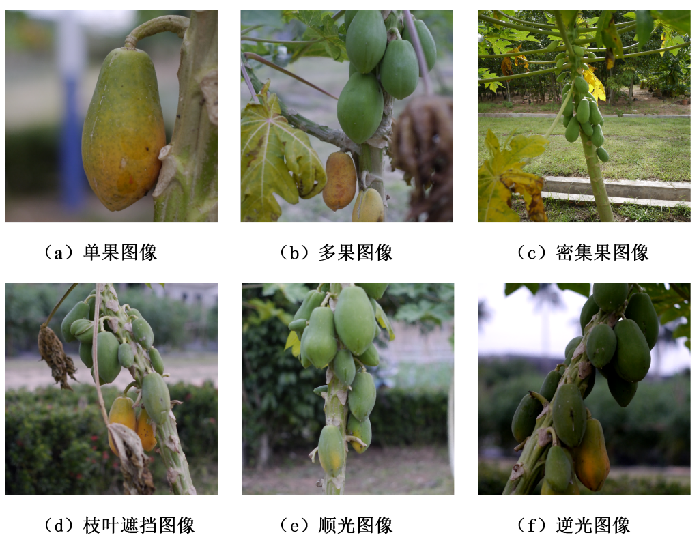
\includegraphics[width=0.75\textwidth]{figures/fig2-1.pdf}
\caption{番木瓜果园采集图像示例}\label{fig:fig2-1}
\vspace{-1em}
\end{figure}


\section{试验环境}


其他网络超参数如表\ref{tab:table2-2}所示。
\begin{table}[h]
    \caption{YOLOv11网络超参数}\label{tab:table2-2}
    \vspace{0.5em}\centering\wuhao
    \begin{tabular}{ll}
    \toprule[1.5pt]
    Hyperparameter & Value \\
    \midrule[1pt]
    每批次图像数量(batch) & 72 \\
    训练轮次(epoch) & 250 \\
    输入图像尺寸(image size) & 640 \\
    动量(momentum) & 0.973 \\
    初始学习率(lr0) & 0.01 \\
    最终学习率(lrf) & 0.01 \\
    权重衰减(weight\_decay) & 0.005 \\
    \bottomrule[1.5pt]
    \end{tabular}
    \vspace{\baselineskip}
    \end{table}

\section{模型评价指标}
计算公式：

（1）准确率：

\begin{equation}
\label{eq:precision}
\mathrm{Precision} = \frac{TP}{TP + FP}
\end{equation}

（2）召回率：
\begin{equation}
\label{eq:recall}
\mathrm{Recall} = \frac{TP}{TP + FN}
\end{equation}


\chapter{结果与分析}
\section{模型改进结果}
这是模型改进结果部分的内容。


\chapter{结论}
这是结论部分的内容。


% \include{mybod}                        
%%%%%%%%%% 致谢  %%%%%%%%%%
% !Mode:: "TeX:UTF-8"

\titlecontents{chapter}[2em]{\vspace{0.25em}\xiaosi\song}
             {{\thecontentslabel}\qquad}{} 
             {\titlerule*[10pt]{.}\contentspage} % 添加页码显示
\addcontentsline{toc}{chapter}{\xiaosi 致\qquad 谢} % 添加到目录中
\chapter*{\makebox[\textwidth][c]{\sanhao\song{\bfseries{ 致\qquad 谢}}}}
% \setcounter{page}{2}
%下面的内容可以根据需要修改(两个回车换行)
行文至此，落笔为终。回首论文写作的整个过程，从选题构思、框架搭建到反复修改，其间既有探索的迷茫，也有顿悟的欣喜。
在此，谨以最诚挚的谢意，向所有给予我帮助和支持的人致以衷心的感谢。

求学四载，终成一文。论文的完成既是一段旅程的终点，亦是人生新程的起点。惟愿以此刻为序，心怀感恩，砥砺前行            % 致谢
%%%%%%%%%%  参考文献  %%%%%%%%%%

\defaultfont
\titleformat{\chapter}{\centering\sanhao\song\bfseries}{\chaptername}{2em}{} % 设置“参考文献”格式
\bibliographystyle{references/ref.buk}
\phantomsection
\markboth{参考文献}{参考文献}
\addcontentsline{toc}{chapter}{参考文献}       % 参考文献加入到目录
% \nocite{*}  %所有参考文献都显示出来
\bibliography{references/reference}

\clearpage
\end{document}                                 % 结束全文
